The base algorithm is a simple implementation of the MCTS algorithm. All the functions related to it are included in the mcts namespace. It takes as a parameter the abstract class \textit{TheGame}, the position (\textit{Bitboard}) to start the search with and an object (\textit{MctsArg}) to set the parameter to the MCTS algorithm such as the time to search on, the depth of the tree, the number of simulations to run and the number of nodes to create in the tree.
The following Class Diagram\ref{fig:MCTSClassDiagram} represent the links between the differents kinds of objects.
\begin{figure}[H] 
\centerline{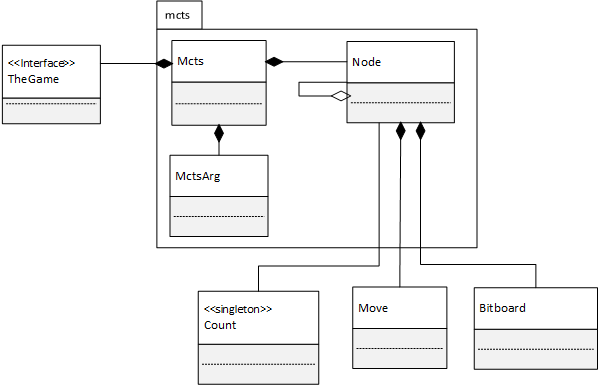
\includegraphics[width=0.6\textwidth]{Base_Algorithm/Img/MCTSsimple.png}}
\caption{\label{fig:MCTSClassDiagram}\textit{Class Diagram of the mcts namespace}}
\end{figure}
The class Node represents the tree, it is stored as an array in the mcts object. A detailed implementation is provided in the Data Structure part.

The singleton \textit{Count} is used for the statistics (such as the number of leaves, nodes created and the number of simultions run). Whilst providing statistics it also makes sure that no  memory leaks are happening, monitoring creations and destructions of the main objects.

The following figure\ref{fig:MCTSAlgorithm} represents the order of the call for the main function while providing some details about the implementation.
\begin{figure}[H]
\centerline{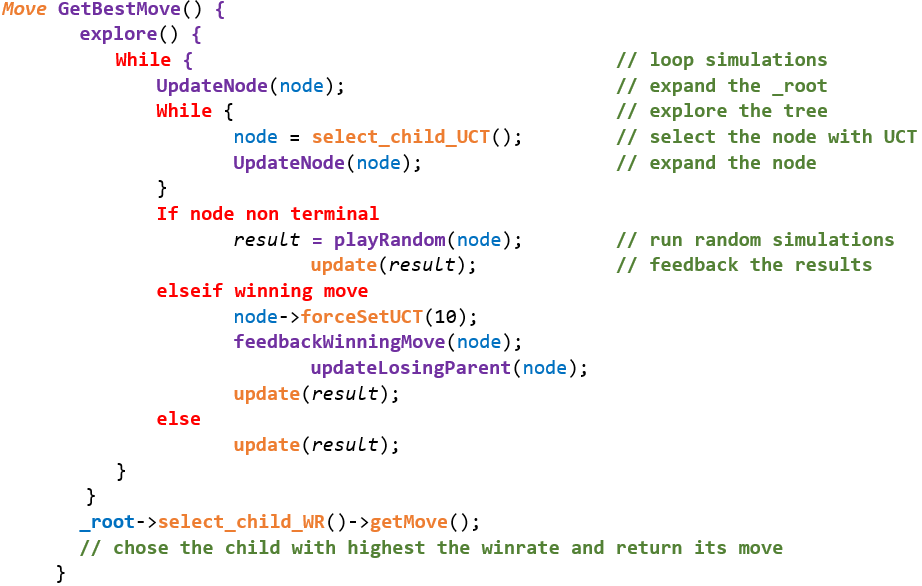
\includegraphics[width=0.7\textwidth]{Base_Algorithm/Img/Algorithm.png}}
\caption{\label{fig:MCTSAlgorithm}\textit{Overview of the implementation of the function GetBestMove()}}
\end{figure}
\noindent
\textit{\textbf{explore}} : start the tree exploration.
\medskip\\
\textit{\textbf{UpdateNode}} : make sure the node has children and update its terminal value if required.
\medskip\\
\textit{\textbf{select\_child\_UCT}} : go through all the children of a node and return the one with the highest result at the UCT function (refer to the \textit{pre-analysis report, part 3.4.4}).
\medskip\\
\textit{\textbf{playRandom}} : start to run the random simulations and return the winner/tie.
\medskip\\
\textit{\textbf{update}} : update the node statistics and feedback the result to its parents.
\medskip\\
\textit{\textbf{forceSetUCT}} : In the event of a winning move, the uct value is set to 10 in order to make sure that each and every further explorations go through that node.
\medskip\\
\textit{\textbf{feedbackWinningMove}} : feedback the winning move to its parent, one does not want to go to that position because it would be a winning strategy for the opponent.
\medskip\\
\textit{\textbf{updateLosingParent}} : in the event of all the siblings being a losing move, update its UCT value to winning strategy in order to propagate the results.
\medskip\\
\textit{\textbf{select\_child\_WR}} : return the child with the highest win rate.\\
